% !TeX spellcheck = cs_CZ
\wikitextrule
\begin{example}\label{MAI:exam025}
  Uvažme funkci z příkladu \ref{fyz:fey_exam017}. 
  
  {\centering
   \captionsetup{type=figure}
%   % !TeX spellcheck = cs_CZ
\documentclass[11pt]{standalone}
\usepackage{xltxtra}
\usepackage[usenames,x11names]{xcolor}
\usepackage{tikz}
\usepackage{pgfplots}
  \pgfplotsset{compat=newest}
\usepackage{amsmath}

\begin{document}
  \begin{tikzpicture}[thick,scale=0.7, every node/.style={transform shape}]
    \begin{axis}[
      xmin = -5, xmax = 5, ymin = -10, ymax = 1.5,
   %   domain = -0.999999:0.999999,
      restrict y to domain=-30:1.5,
      unit vector ratio=1 1 1,  % axis equal
      grid = both,   % both, major
      grid style={line width=.1pt, draw=gray!20},
      major grid style={dashed, line width=.2pt, draw=gray!40},
      minor tick num=4,
      clip = true,
      clip mode=individual,
      axis x line = middle,
      axis y line = middle,
      xlabel={$x$},
    %  xlabel style={at=(current axis.right of origin), anchor=west},
      ylabel={$u,w,y$},
    %  ylabel style={at=(current axis.above origin), anchor=south},
      enlarge y limits={rel=0.13},
      enlarge x limits={rel=0.07},
    ]
    
      \addplot[color=Gold3, samples=1000, smooth, ultra thick, unbounded coords=jump, no markers, 
               domain = -0.999999:0.999999] 
        gnuplot{log10(sqrt(1-x^2))/log10(2)};  
        
     \addplot[color=green, samples=200, smooth, ultra thick, unbounded coords=jump, no markers, 
     domain = -3.3:3.3] 
        gnuplot{1-x^2};
        
     \addplot[color=blue, samples=200, smooth, ultra thick, unbounded coords=jump, no markers, 
     domain = -1:1] 
        gnuplot{sqrt(1-x^2)};  
    \end{axis}
  \end{tikzpicture}
\end{document}
   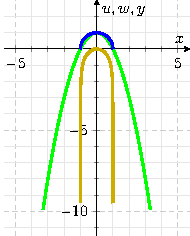
\includegraphics[width=0.45\linewidth]{mai_fig013.pdf}
   \captionof{figure}{K příkladu \ref{MAI:exam025} \(y=\log_2{(\sqrt{1-x^2})}\) 
   \cite[s.~57]{Musilova2009MA1}
   \label{mai:fig013}}
  \par}
  
  Ukážeme, jak tato funkce vzniká postupně složením tří funkcí a jak při tom dochází k postupnému 
  omezování definičního oboru. Písmeny \(\mathcal{D}\) a \(H\) s příslušným indexem budeme značit 
  definiční obory a obory hodnot jednotlivých funkcí.
  \begin{align*}
    g&:  \realset =\mathcal{D}_g\ni x\rightarrow u=g(x) = 1- x^2  \in\mathcal{H}_g=(-\infty,1], \\
    h&: [0,\infty)=\mathcal{D}_h\ni u\rightarrow w=h(u) = \sqrt{u}\in\mathcal{H}_h=[0,\infty),
  \end{align*}
  \begin{equation*}
    \mathcal{D}_h\cap\mathcal{H}_g = [0,1]\Rightarrow\mathcal{D}_{h\circ g}=[-1,1], 
    \mathcal{H}_{h\circ g} = [0,1], 
  \end{equation*}
  \begin{equation*}
    f:(0,\infty)=\mathcal{D}_f\ni w \rightarrow y=f(w)=\log_2w\in\mathcal{H}_f=\realset
  \end{equation*}
  \begin{equation*}
    \mathcal{H}_{h\circ g}\cap\mathcal{D}_f = (0,1] 
    \Rightarrow\mathcal{D}_F=(-1,1),\mathcal{H}_F=(-\infty,0]. 
  \end{equation*}
  Je tedy
  \begin{align*}
    F:\mathcal{D}_F\ni x\rightarrow 
    y&=F(x)=(f\circ(h\circ g))(x) = f{h[g(x)]}          \\
     &= \log_2\sqrt{1-x^2}\in(-\infty,0].
  \end{align*}
  Názorněji než tento zápis ukazuje situaci obrázek \ref{mai:fig013}.
\end{example}